\chapter{Method of Investigation}
A study requires a methodology to minimize errors in decision making. This chapter describes systematically the overview of the methodology used in this study. The steps performed are shown in figure \ref{fig:research_methodology_flow_diagram_1} and \ref{fig:research_methodology_flow_diagram_2} below :

\begin{figure}[H]
    \centering
    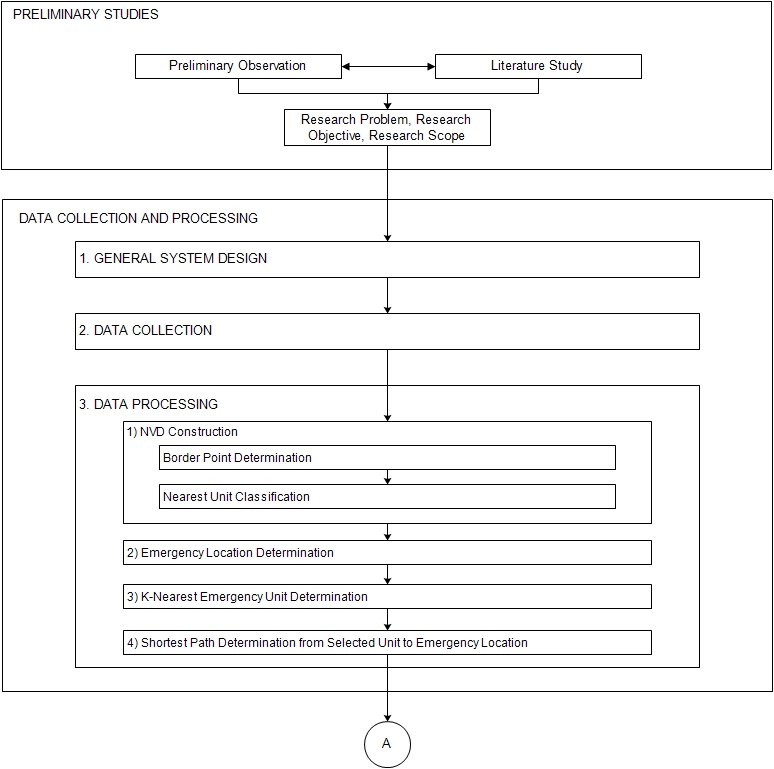
\includegraphics[scale=0.65]{flow_diagram_metodologi_penelitian_1.jpg}
    \caption{Methodology Flow Diagram (1)}
    \label{fig:research_methodology_flow_diagram_1}
\end{figure}

\begin{figure}[H]
    \centering
    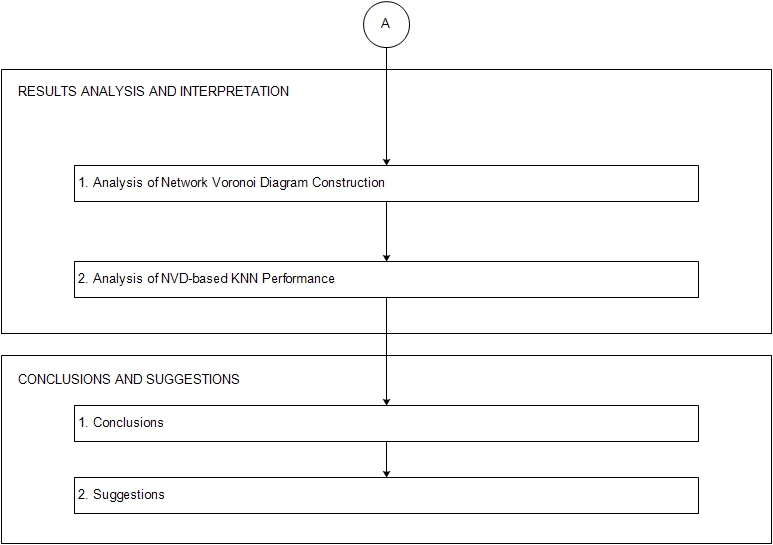
\includegraphics[scale=0.65]{flow_diagram_metodologi_penelitian_2.jpg}
    \caption{Methodology Flow Diagram (2)}
    \label{fig:research_methodology_flow_diagram_2}
\end{figure}

\section{Preliminary Studies}
Initial observations are made by observation to the field directly. Field observation process provides an overview of the problems that exist, then this problem put together into the formulation of the problem. Formulation of problems that arise that is how to determine the nearest emergency unit from emergency location and compute route to it based on the shortest path.

This literature study was conducted to support the process for this study. Some of the literature used are the study of first aid emergency, the study of network voronoi diagram, the study of k-nearest neighbor, and analysis of the road network using geographic information system. Sources of literature comes from books, journals, previous study related, and also sources of information from the internet.
\pagebreak

\section{General System Design}
The purpose of system design in general is to provide a general overview of the system built and identify the components of the systems that will be designed in detail.

\subsection{System Description}
The system built on this research is the first aid emergency system by using Network Voronoi Diagram based K-Nearest Neigbor. In general, the system can be seen in figure \ref{fig:system_description} below. First, system accepts input user location where emergency happens. Then the system will process the input to determine nearest emergency units to emergency location that has been divide using Network Voronoi Diagram. If the selected unit is on duty, system will looking for next nearest emergency unit using K-Nearest Neighbor. After k-nearest emergency unit selected, system determines the shortest path from their location to emergency location. And the last, system sends data to the results of this process to each selected emergency unit so that they can immediately go to the emergency location to do first aid.

\begin{figure}[H]
    \centering
    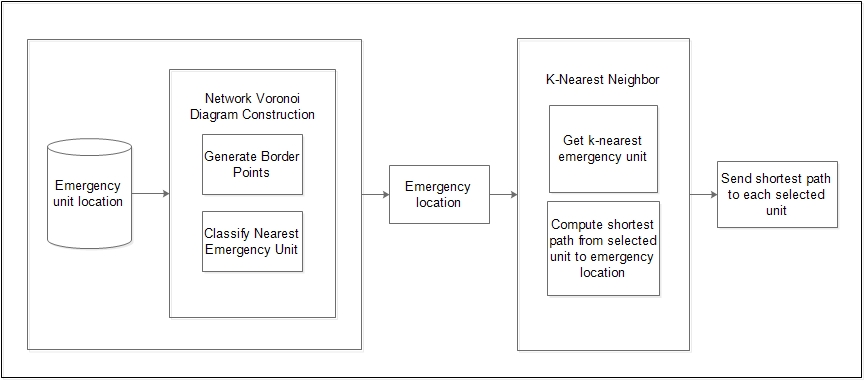
\includegraphics[scale=0.6]{system-desc.jpg}
    \caption{System Description}
    \label{fig:system_description}
\end{figure}
\pagebreak

\subsection{System Flowchart}

\begin{figure}[H]
    \centering
    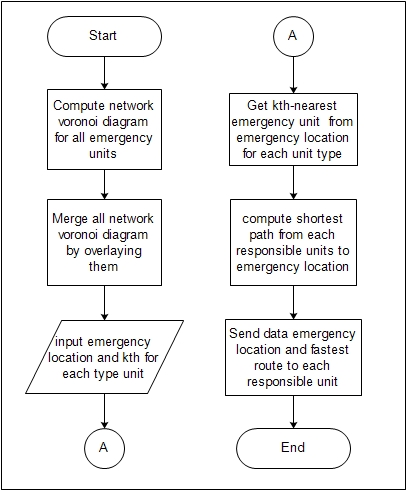
\includegraphics[scale=0.7]{system-flow.jpg}
    \caption{System Flowchart}
    \label{fig:system_flowchart}
\end{figure}


\begin{enumerate}[leftmargin=*, topsep=5pt, itemsep=-1ex, partopsep=1ex, parsep=2ex]
	\item System determining border points for all emergency units as a middle point between adjacent units.
    \item System construct network voronoi diagram to get each vertex perspective about its nearest emergency unit so it will make a territory for each unit in same unit type.
    \item System merge all network voronoi diagram (nvd for ambulance, nvd for police, and nvd for fire brigade), which has been constructed by overlaying all of them.
    \item System gets emergency location inputs where emergency occurs.
    \item System determining nearest unit to emergency location. If selected unit is on duty, system will looking into next nearest unit. Until system find it an appoint it as responsible unit.
    \item System compute shortest path from each responsible units to emergency location.
    \item System sends data emergency coordinates location and shortest path from each responsible units to the location.
\end{enumerate}
\pagebreak


\section{Data Collection and Processing}
Data collection and processing are used to get the final result of the nearest emergency units(police, ambulance, fire brigade) from emergency location (traffic accident) and compute route to it.

\subsection{Data Collection}
Data collection needed as support for determining nearest emergency unit from emergency location. The data collected are:

\begin{enumerate}[label=- , leftmargin=*, topsep=5pt, itemsep=-1ex, partopsep=1ex, parsep=2ex]
\item Bandung road network map\\
These map contains some public road network in Bandung City partially including south side, west side, east side, and center side. The public road network includes arteries and collector road type.
\item Coordinate location data of ambulance units\\
These coordinate location data of ambulance units are obtained from portal data Bandung.
\item Coordinate location data of police units\\
These coordinate location data of police units are obtained from Kepala Polisi Resor Bandung and portal data Bandung.
\item Coordinate location data of fire brigade units\\
The coordinate location data of police units are obtained from Dinas Pemadam Kebakaran Bandung and portal data Bandung.
\end{enumerate}

\subsection{Data Processing}
Data processing step serves to find responsible units and generate shortest path from them to emergency location. This step can be explained as follows:

\subsubsection{3.3.3.2.1 Process of Constructing NVD}
This step works by divide Bandung into coverage area for each emergency unit. The coverage area denotes that every location inside the coverage area will return its emergency unit as nearest emergency unit. NVD construction also looking for neighborhoods between adjacent emergency unit which used for searching next nearest emergency unit. NVD Construction consists of the process of determining border points and process of nearest unit classification.

\pagebreak

\subsubsection{Process of Determining Border Point}
\begin{enumerate}[label=Input\hspace{5mm} :\hspace{2mm}, leftmargin=*, topsep=0pt, itemsep=-1ex, partopsep=1ex, parsep=1ex]
\item road network, ambulance units coordinate point, police units coordinate point, fire brigade units coordinate point
\end{enumerate}
\begin{enumerate}[label=Output\hspace{2mm} :\hspace{2mm}, leftmargin=*, topsep=0pt, itemsep=-1ex, partopsep=1ex, parsep=1ex]
\item ambulance units border point, police border point, fire brigade border point
\end{enumerate}
Border point denotes middle distance from two adjacent emergency units. Border point will act as outer parts from a emergency unit's territory. To determining border points, system needs to read road network and also coordinate point of each emergency unit. After system reads the input, each emergency units will be selected as starting point and expand to other vertex which share same edge with them. Border point obtained when expanding process meets another emergency unit.

\begin{figure}[H]
    \centering
    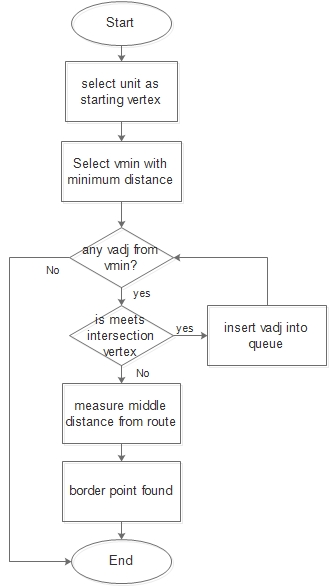
\includegraphics[scale=0.8]{flowchart_bp.jpg}
    \caption{Flowchart Border Point Determination}
    \label{fig:bp_pol}
\end{figure}

\pagebreak
\subsubsection{Process of Classifying nearest unit}
\begin{enumerate}[label=Input\hspace{5mm} :\hspace{2mm}, leftmargin=*, topsep=0pt, itemsep=-1ex, partopsep=1ex, parsep=1ex]
\item road network, ambulance units coordinate point, ambulance units border point, police units coordinate point, police units border point, fire brigade units coordinate point, fire brigade units border point
\end{enumerate}
\begin{enumerate}[label=Output\hspace{2mm} :\hspace{2mm}, leftmargin=*, topsep=0pt, itemsep=-1ex, partopsep=1ex, parsep=1ex]
\item ambulance units network voronoi diagram, police network voronoi diagram, fire brigade network voronoi diagram
\end{enumerate}
This step works by classifying nearest generator (1-NN) for each vertex in plane. Network voronoi diagram will shows territory of each unit in same type. To construct NVD, system needs to read road network and all vertex including generator, border points, or normal vertex. This process will be computed three times because there are three types of units (police, ambulance, fire brigade).

\begin{figure}[H]
    \centering
    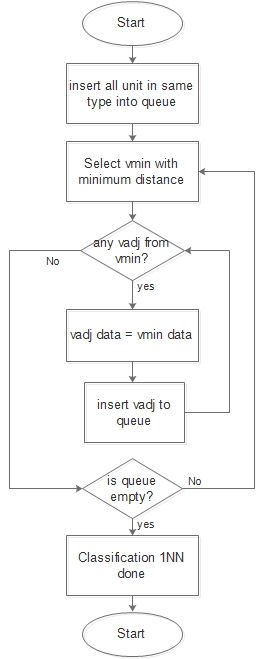
\includegraphics[scale=0.75]{flowchart_classify.jpg}
    \caption{Flowchart Nearest Unit Classification}
    \label{fig:bp_pol}
\end{figure}

\pagebreak
\subsubsection{3.3.3.2.2 Process of Determining Emergency Location}
\begin{enumerate}[label=Input\hspace{5mm} :\hspace{2mm}, leftmargin=*, topsep=0pt, itemsep=-1ex, parsep=1ex]
\item emergency coordinate location
\end{enumerate}
\begin{enumerate}[label=Output\hspace{2mm} :\hspace{2mm}, leftmargin=*, topsep=0pt, itemsep=-1ex, parsep=1ex]
\item map with emergency location
\end{enumerate}
This step is works by determining coordinates of emergency location based on emergency request. When emergency call comes, network connectivity points (e.g., cellular towers of cellular networks) will detect user coordinate location and report it to emergency service system. The emergency location become endpoint in route determination to finding shortest path from selected unit.

\subsubsection{3.3.3.2.3 Process of Determining K-Nearest Emergency Unit}
\begin{enumerate}[label=Input\hspace{5mm} :\hspace{2mm}, leftmargin=*, topsep=0pt, itemsep=-1ex, parsep=1ex]
\item emergency coordinate location, k-selected
\end{enumerate}
\begin{enumerate}[label=Output\hspace{2mm} :\hspace{2mm}, leftmargin=*, topsep=0pt, itemsep=-1ex, parsep=1ex]
\item selected unit
\end{enumerate}
This step intended to selecting number of k for type unit which emergency needed. If the nearest unit on duty, system will determine next nearest unit with adjacency generator list as control. The nearest emergency unit's neighbour becomes candidate to next nearest unit. These candidates will sorted by minimum distance to emergency location. Then, system pick up k-nearest emergency unit to emergency location The selected unit will become starting point in route determination.

\begin{figure}[H]
    \centering
    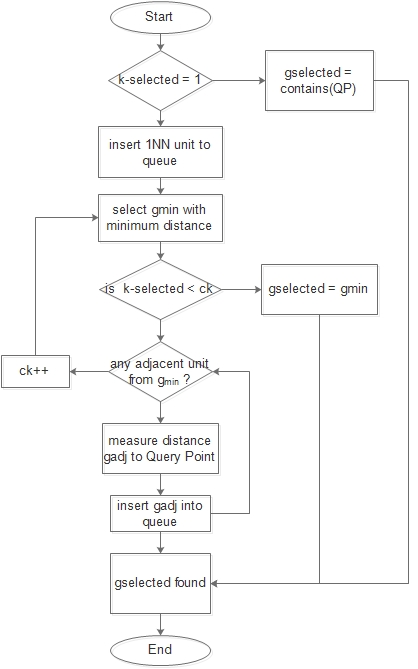
\includegraphics[scale=0.56]{flowchart_knn.jpg}
    \caption{Flowchart K-Nearest Emergency Unit Determination}
    \label{fig:bp_pol}
\end{figure}

\pagebreak
\subsubsection{3.3.3.2.4 Process of Determining Shortest Path from Selected Emergency Unit to Emergency Location}
\begin{enumerate}[label=Input\hspace{5mm} :\hspace{2mm}, leftmargin=*, topsep=0pt, itemsep=-1ex, parsep=1ex]
\item selected unit location, emergency location
\end{enumerate}
\begin{enumerate}[label=Output\hspace{2mm} :\hspace{2mm}, leftmargin=*, topsep=0pt, itemsep=-1ex, parsep=1ex]
\item nearest route
\end{enumerate}
This step used to send shortest path information to selected emergency units so they can immediately do first aid. It will reduce or even prevent fatal impact from emergency. These selected unit will becomes starting point and the emergency location will becomes end point. System will expanding road network and select vertex with minimum distance from starting point to end point.

\section{Analysis and Interpretation Data}
In this section, data analysis and interpretation of the results based on data collection and processing in the previous section. The purpose of this section is to provide clearer information about the results and able to provide solutions to emerging research problems.


\subsection{Analysis of NVD Construction}
Analysis of NVD construction results is used to determine coverage area of each emergency unit to determine nearest emergency unit from an emergency location.

\subsection{Analysis of NVD-based KNN Performance}
The result of k-nearest emergency unit analysis is done to show the performance of accuracy and execution time between NVD-based KNN and basic KNN in case determining k-nearest emergency unit.


\section{Conclusions and Suggestion}
The conclusions and suggestions step is the final step of this final project which contains the conclusions of the overall results and analysis that refers to the initial objectives. It also provides advice related to the development that can be built for further research.